\documentclass[aspectratio=169,11pt]{beamer}
\usetheme{Madrid}
\usepackage{amsmath, amssymb}
\usepackage{graphicx}
\usepackage{tikz}
\usepackage{comment}
\usepackage{hyperref}
\usepackage{subcaption}

\graphicspath{{figures/}}

\newcommand{\sectionframe}[1]{%
  \begin{frame}[plain]
    \centering
    \vfill
    {\Huge #1}
    \vfill
  \end{frame}
}

\title[]{Learning Dynamics}
\author[Corlouer]{Guillaume Corlouer}
\institute{Stormglass}
\date{}

\begin{document}
\maketitle
\begin{frame}{Big questions}
\begin{itemize}
    \item How a model generalize
    \item Internal structure formation during training
    \item Emergent capabilities
    \item Control levers of the training process
    \item How loss, architecture, data, optimizer determinate how internal structure is learned throughout training
\end{itemize}
\end{frame}
\begin{frame}{How: making mathematical models of learning}
    \begin{itemize}
        \item Tractable toy models: deep linear networks, shallow non linear networks, polynomial activations
        \item Take limits: depth, width, data, training time
        \item Exploit symmetries: quotient them out, find conserved quantities
        \item Identify useful coarse grained variables: singular values of weights, learning coefficient, correlation functions
        \item Work in specific regimes: lazy vs rich
        \item Validate with tight feedback loops: run experiments, symbolic derivations, mathematical proofs
    \end{itemize}
\end{frame}
\begin{frame}{Safety motivations}
    \begin{itemize}
        \item A central question in AI safety is wether the training process select a harmful model (scheming, sycophantic, spiteful...)
        \item Predict if a model is going to be harmful in high stakes and out of distribution environment while behavioural or average case interpretability evals cannot be trusted
        \item Develop stronger interpretability methods by decomposing throughout training
        \item We want a mathematical model that can beat average methods at predicting harmful behaviour
        \item More ambitiously we would like to find control levers of the training process to be confident that training will select a safe model
    \end{itemize}
\end{frame}
\section{Setup}
\begin{frame}[plain]
\begin{tikzpicture}[remember picture,overlay]
\node[inner sep=0pt] at (current page.center) {%
\begin{beamercolorbox}[wd=.75\paperwidth,sep=1.4em,center,rounded=true,shadow=true]{title}
{\usebeamerfont{title}\Huge Setup}
\end{beamercolorbox}
};
\end{tikzpicture}
\end{frame}
\begin{frame}{Deep neural network}
\begin{columns}[T,onlytextwidth]
\begin{column}{0.48\textwidth}
Let parameter $\theta\in \Omega$, input $x\in\mathbb{R}^{d_0}$, weight matrices $W_l\in\mathbb{R}^{d_l \times d_{l+1}}$, activation function $\sigma$:
\[
h_l(\theta,x) = \sigma(W_lh_{l-1} + b_l)
\]
A neural network is a function $f$ such that:
\[
f(\theta, x) = W_Lh_{L-1}(\theta,x)
\]
Other architectural components: residual stream, tokenization, embeddings, attention for sequence modeling, layer normalization...
\end{column}
\begin{column}{0.48\textwidth}
\centering
\vspace{0.2cm}
\resizebox{\linewidth}{!}{\input{figures/deep_neural_network.tex}}
\end{column}
\end{columns}
\end{frame}
\begin{frame}{Deep Linear Network}
Function is linear in data, non linear in parameters:
  \[
    \begin{aligned}
      f: \ & \mathbb{R}^{d_0} \times \prod_{l=0}^{L-1}\mathbb{R}^{d_l \times d_{l+1}}  \to \mathbb{R}^{d_L} \\
         & (x,W_1,...,W_L) \mapsto W_L...W_1 x = Wx
    \end{aligned}
  \]
$d_0$ is the input dimension; $d_\ell$, $1\leq \ell \leq L$, is the width of layer $\ell$.
Define the product map:
\[
\mu(\theta) := W_L...W_1 = W
\]
Where $W$ is the student matrix.
\end{frame}
\begin{frame}{Stochastic gradient descent}
Learn a function $g$ from observing $y = g(x)$. Initialize neural weights at $\theta_0 \sim N(0,\sigma^{-\gamma})$ with initialization scale $\gamma$. 
\begin{block}{SGD update}
    Consider dataset of size $N$. At each time step sample batch $b$ of size $B$. Empirical loss and batch loss relation:
\[
\mathcal{L}(\theta) = \langle \mathcal{L}(\theta; b)\rangle_b
\]
    SGD updates is:
\[
\theta_{k+1} = -\eta\nabla_{\theta_k}\mathcal{L}(\theta_k) + \eta \xi(\theta_k, b_k)
\] 
With gradient noise 
\[
\xi(\theta, b):= \nabla \mathcal{L}(\theta_k) - \nabla \mathcal{L}(\theta_k; b_k) 
\]
\end{block}
Loss function $\mathcal{L}$ can for example be mean square error or cross entropy loss
\end{frame}
\begin{frame}{Data, loss function, gradient flow}
\begin{block}{Quadratic population loss and gradient flow}
Let $M$ be the teacher matrix, with $y=Mx$ and $x\sim \mathcal{N}(0,I)$.
The input-output covariance is $\Sigma_{YX}=M$.
\begin{equation*}
    \mathcal{L}(\theta) := \frac{1}{2} \lVert M - W_L\cdots W_1\rVert^2_F = \frac{1}{2} \lVert M - W\rVert^2_F
\end{equation*}
Initialize $\theta_0 \sim \mathcal{N}(0, \sigma^{-\gamma})$, where $\gamma$ controls the initialization scale. Then gradient flow is
\[
\dot{W}_\ell = - \nabla_{W_{\ell}} \mathcal{L}(\theta).
\]
\end{block}
Frobenius norm: $\lVert A\rVert_F:=\sqrt{\operatorname{Tr}(A^{\top}A)}$.
\\
Global minimizers achieve zero loss: $\exists \theta^{\star}\in \Omega,\ \mu(\theta^{\star}) = W^{\star} = M$.
\\
The structure of the data is encoded by $\Sigma_{YX}$.
\end{frame}
\begin{frame}
    \centering Geometry
\end{frame}
\begin{frame}[plain]
\centering
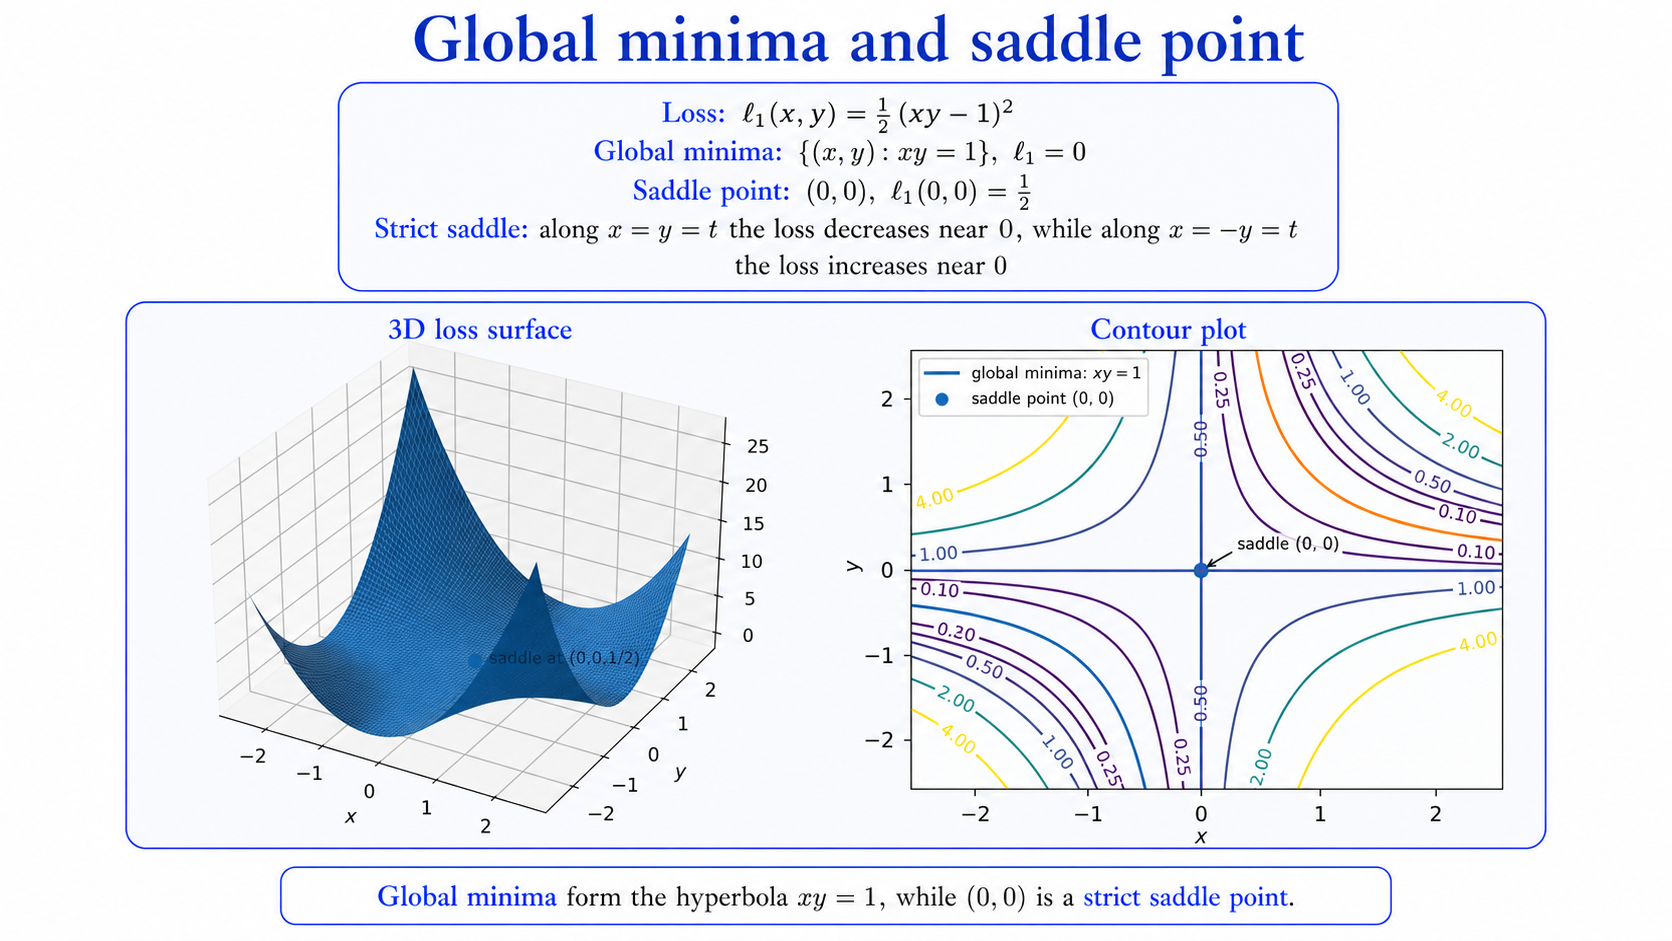
\includegraphics[width=\textwidth,height=\textheight,keepaspectratio]{figures/global_minima_saddle_3d_loss.png}
\end{frame}
\begin{frame}{Deep learning without poor local minima}
Assume that $\Sigma_X$ and $\Sigma_{YX}$ are full rank, and that $\Sigma_{YX}$ has $d_L$ distinct singular values.
\begin{block}{No non-global local minima}
    The loss function of a DLN of depth $L$ is non-convex and non-concave, and every critical point that is not a global minimum is a saddle point.
\end{block}
The training dynamics cannot get stuck in spurious local minima.
\\
Reference: \textit{Kawaguchi, Kenji. "Deep learning without poor local minima." Advances in neural information processing systems 29 (2016)}
\end{frame}
\begin{frame}{Parametrization of critical points}
Teacher SVD: \(M=U\operatorname{diag}(s_1,\ldots,s_{r_m},0_{d_L-r_m})V^{\top}\).
\begin{block}{Saddle points}
    Let $\theta\in\Omega$ be a critical point of rank $r$. Then there exists a subset $S$ of left singular vectors of $M$ and a projector $P_S=U_S U_S^{\top}$ onto their span such that:
    \[
    \mu(\theta) = P_S M = U_S\operatorname{diag}(s_1,\ldots,s_{r},0_{d_L-r})V^{\top}
    \]
\end{block}
The saddle points are given by a subset of singular values and (left) singular vectors of the teacher $M$.
\\
Reference: \textit{Achour, El Mehdi, François Malgouyres, and Sébastien Gerchinovitz. "The loss landscape of deep linear neural networks: a second-order analysis." Journal of Machine Learning Research 25.242 (2024): 1-76.}
\end{frame}
\begin{frame}{Symmetries}
Let $G_{\mathbf{d}}:=\prod_{\ell=0}^{L} GL_{d_\ell}$ act on $\Omega$ via:
\[
(W_1,\dots,W_L)\mapsto (g_1W_1g_0^{-1},\; g_2W_2g_1^{-1},\;\dots,\; g_L W_L g_{L-1}^{-1}),
\]
\begin{block}{Equivariance of the multiplication map}
    Since \(W_Lg_{L-1}^{-1}g_{L-1}W_{L-1}\cdots g_1^{-1}g_1W_1=W_L\cdots W_1\), the multiplication map $\mu$ is $G_{\mathbf{d}}$-equivariant and $G_h$-invariant:
    \[
    \mu(g\cdot \theta)=g_L W g_0^{-1},
    \qquad
    \mu(g_h\cdot \theta) = \mu(\theta).
    \]
A DLN is degenerate: infinitely many DLNs can map to the same student matrix.
\end{block}
It is natural to study solutions up to $G_d$ symmetries. By equivariance of $\mu$, $G_d$ acts on the determinantal variety
\[
\Sigma_d^{r}:=\{\theta\in \Omega\mid\operatorname{rank}(\mu(\theta)) = r\}.
\]
\end{frame}
\begin{frame}{Stratification of the fiber of the parameter function map}
\begin{block}{Orbits are parameterized by rank patterns}
The $G_d$-orbits in $\Sigma_d^r$ are indexed by rank patterns $\rho_{ij}=\text{rank}(W_j...W_i)$:
\[
\Sigma_d^r = \bigsqcup_{\rho_{ij}} \mathcal{O}_{\rho}
\]
Two DLN are in the same $G_d$-orbit if and only if they have the same rank pattern
\\
 Since $\Sigma_d^{r} = G_{\text{out}}\cdot\mu^{-1}(W)$, this gives a combinatorial description of the fiber of the product map $\mu^{-1}(W)$
\end{block}
Rank patterns are natural observables from geometric invariants for DLNs.
\end{frame}
\begin{frame}{Link with SLT}
\begin{block}{Codimension of the global minima}
For a teacher matrix $M$ of rank $r_m$, we have:
    \[
    \begin{aligned}
    \operatorname{codim}(\mu^{-1}(M))
    &=
    \operatorname{codim}(\Sigma_d^{r_m})
    + r_m(d_0 - d_L - r_m) \\
    &= 2\operatorname{RLCT}(\mathcal{L}^{-1})(0).
    \end{aligned}
    \]
In general, we only have:
\[
\operatorname{RLCT}(\mathcal{L}^{-1})(0)  \leq \frac{1}{2}\operatorname{codim}_{\operatorname{Rep}_d}(\mathcal{L}^{-1}(0)).
\]
\end{block}
Ref: \textit{Lehalleur, Simon Pepin, and Richárd Rimányi. "Geometry of fibers of the multiplication map of deep linear neural networks." arXiv preprint arXiv:2411.19920 (2024).}
\end{frame}
\begin{frame}{Discussion}
\begin{block}{Takeaways}
Under full-rank and nondegenerate-data assumptions:
    \begin{itemize}
        \item Critical points of DLNs are either saddles or global minima
        \item Gauge symmetries mean there is a whole algebraic variety of degenerate minima
        \item Geometric invariants give observables and a combinatorial description of the parameter function map and the global minima
    \end{itemize}
\end{block}
\end{frame}
\begin{frame}{References}
\begin{itemize}
    \item Kenji Kawaguchi. Deep learning without poor local minima \textit{Advances in neural
information processing systems}, 29, 2016.
    \item El Mehdi Achour, François Malgouyres, and Sébastien Gerchinovitz. The loss
landscape of deep linear neural networks: a second-order analysis. \textit{Journal of
Machine Learning Research}, 25(242):1–76, 2024.
    \item Anna Choromanska, Mikael Henaff, Michael Mathieu, Gérard Ben Arous, and
Yann LeCun. The loss surfaces of multilayer networks. In \textit{Artificial intelligence
and statistics}, pages 192–204. PMLR, 2015.
    \item Lehalleur, Simon Pepin and Rim{\'a}nyi, Rich{\'a}rd. Geometry of fibers of the multiplication map of deep linear neural networks, arXiv preprint arXiv:2411.19920, 2024.
    \item Chen, Po and Jiang, Rujun and Wang, Peng. A Complete Loss Landscape Analysis of Regularized Deep Matrix Factorization, arXiv preprint arXiv:2506.20344, 2025.
\end{itemize}
\end{frame}
\begin{frame}
    \begin{center}
        Dynamics 
    \end{center}
\end{frame}
\begin{frame}{Gradient flow and NTK dynamics}
  \small
  Small-learning-rate limit of gradient descent:
  \[
    \theta_{t+1}=\theta_t-\eta \nabla_\theta \mathcal{L}(\theta_t)
    \qquad \leadsto \qquad
    \dot{\theta}(t)=-\nabla_\theta \mathcal{L}(\theta(t))
  \]

  Neural Tangent Kernel (NTK):
  \[
    K(x,x',\theta) =
    \nabla_{\theta} f(\theta, x) \nabla_{\theta} f^{\top}(\theta, x) =
    \sum_{i=1}^p \partial_{\theta_i} f(\theta, x) \partial_{\theta_i} f^{\top}(\theta, x)
  \]

  For a quadratic loss on a dataset $(x_i,y_i)$, the dynamics in function space are
  \[
    \frac{d}{dt}f(\theta, x)
    = -\sum_{i=1}^N K_{\theta}(x,x_i)\big(f_{\theta}(x_i,t)-y_i\big)
  \]
\end{frame}
\begin{frame}{Conserved quantities in DLNs}
  Conserved quantities under gradient flow:
  \[
    G_l = W_{l+1}^{\top}W_{l+1} - W_{l}W_{l}^{\top}
  \]

  When $\beta_l=0$ we have \textbf{balanced weights}

  \vspace{0.4cm}

  For a 1D, 2-layer DLN, we get a hyperbolic equation: $w_2^2 - w_1^2 = \beta$

  \vspace{0.4cm}
\end{frame}
\begin{frame}[plain]
\centering
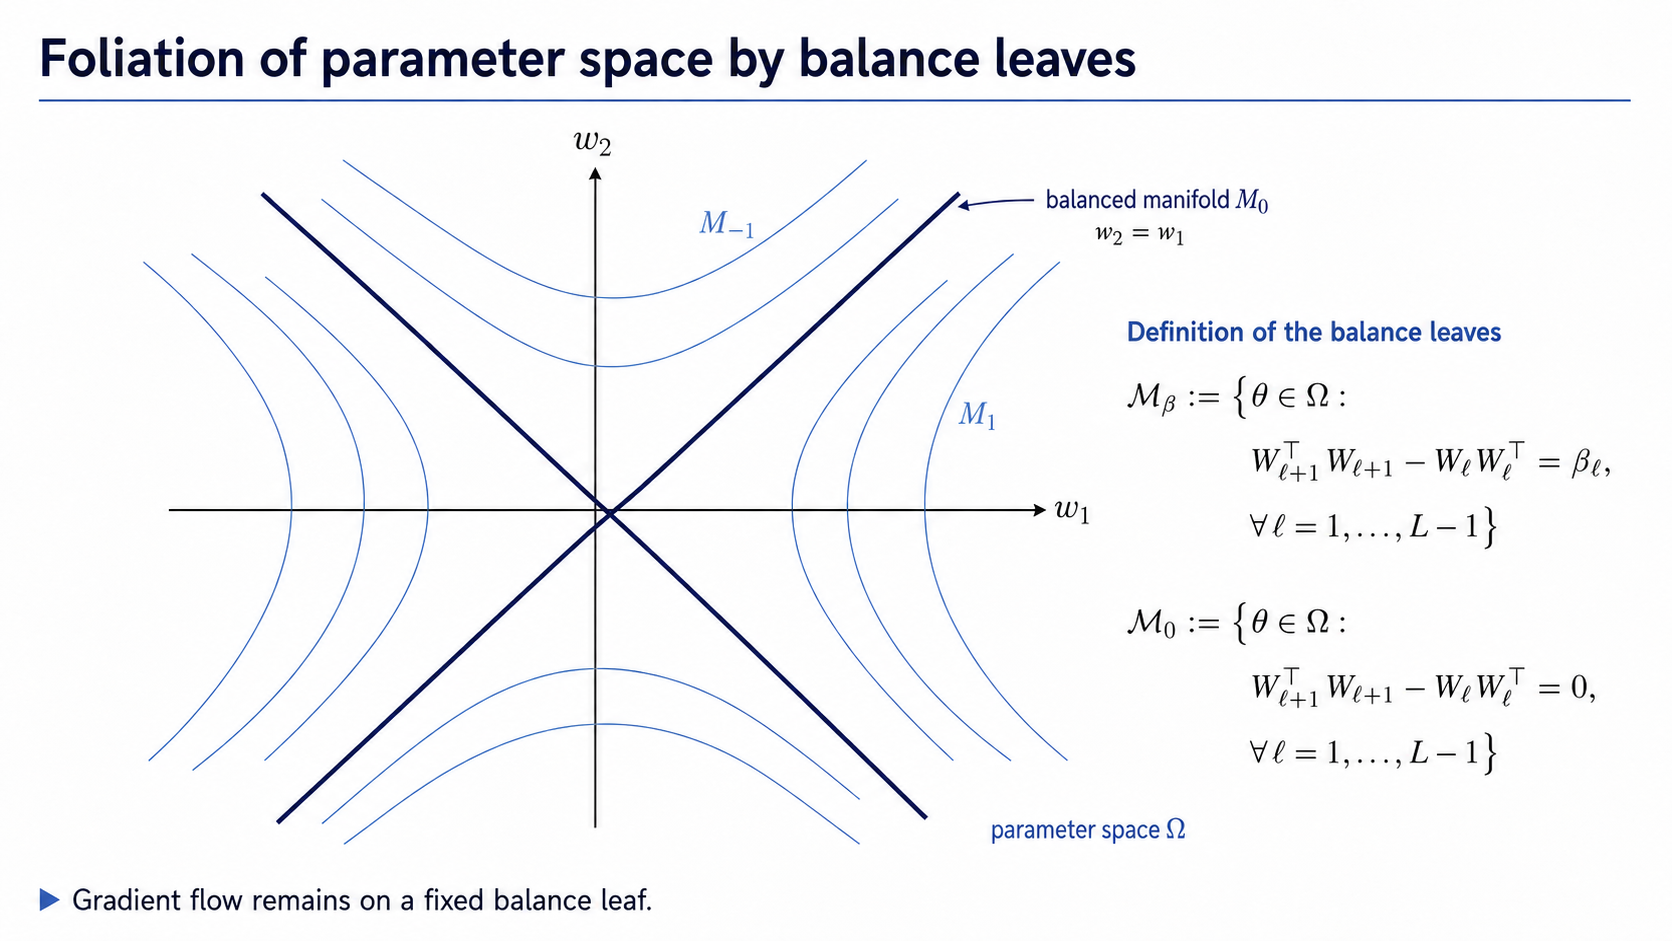
\includegraphics[width=\textwidth,height=\textheight,keepaspectratio]{figures/foliation_paramaters_balanced.png}
\end{frame}
\begin{frame}{The manifold of gradient flow}
Gradient flow is constrained on the following hyperbolic manifold:
\begin{equation*}
    \mathcal{M}_{\beta} := \{\theta\in\Omega\mid W_{\ell+1}^{\top}W_{\ell+1} - W_{\ell}W_{\ell}^{\top} = \beta_\ell\}
\end{equation*}
\begin{block}{Gradient flow on the balanced variety}
On the balanced variety $\mathcal{M}_0$, the self-consistent gradient flow equation in function space is
\begin{equation*}
    \dot{W}
    =
    \sum_{k=1}^{L}
    (WW^{\top})^{\frac{L-k}{L}}
    R(W)
    (W^{\top}W)^{\frac{k-1}{L}},
    \qquad
    R(W):=\Sigma_{YX}-W.
\end{equation*}
For depth $2$:
\[
    \mathcal{M}_0
    =
    \{(W_1,W_2)\mid W_2^{\top}W_2=W_1W_1^{\top}\}.
\]
\begin{equation*}
    \dot{W}
    =
    (WW^{\top})^{\frac{1}{2}}R(W)
    +
    R(W)(W^{\top}W)^{\frac{1}{2}}.
\end{equation*}
\end{block}
\end{frame}
\begin{frame}{Learning rate: Edge of stability}
Descent lemma: For convex loss, loss decreases if $\eta < 2/L$
\\ 
The loss is non-convex, but the Hessian oscillates slightly above $\frac{2}{\eta}$: it regularizes away sharp minima

  \centering
  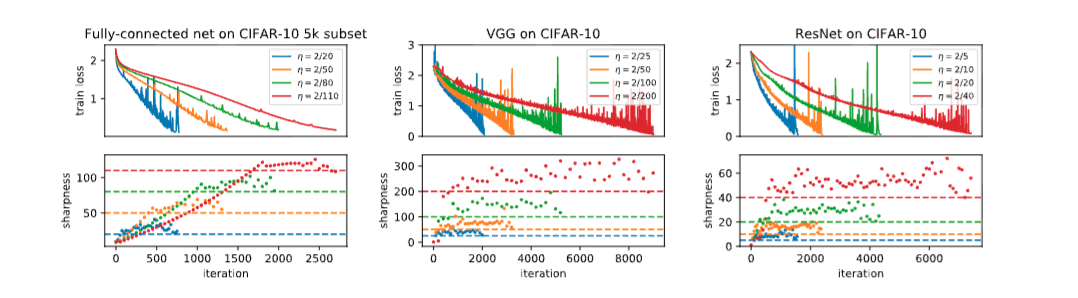
\includegraphics[width=\textwidth,height=0.57\textheight,keepaspectratio]{figures/edge_of_stability.png}


  \begin{minipage}{0.95\textwidth}
    \centering
    Ref: \href{https://arxiv.org/abs/2103.00065}{Gradient Descent on Neural Networks Typically Occurs at the Edge of Stability, Cohen et al.}
  \end{minipage}
\end{frame}
\begin{frame}{Takeaways}
  \begin{block}{Key points}
    \begin{itemize}
      \item NTK preconditions gradient flow in function space
      \item Symmetries can induce conserved quantites which constrain the gradient flow
      \item Gradient flow in function space for balanced quantities lead to self consistent equations
      \item The effect of learning rate can be understood via the edge of stability
    \end{itemize}
  \end{block}
\end{frame}
\begin{frame}{References}
    \begin{itemize}
        \item Menon, Govind. The geometry of the deep linear network. Symposium on Probability and Stochastic Processes. Cham: Springer Nature Switzerland, 2023.
        \item Sibylle Marcotte, R\'emi Gribonval, and Gabriel Peyr\'e. Abide by the law and
follow the flow: Conservation laws for gradient flows. \textit{Advances in neural
information processing systems}, 36:63210–63221, 2023.
    \item Sanjeev Arora, Nadav Cohen, Noah Golowich, and Wei Hu. \textit{A convergence
analysis of gradient descent for deep linear neural networks}. arXiv preprint
arXiv:1810.02281, 2018
    \item Arthur Jacot, Franck Gabriel, and Cl\'ement Hongler. Neural tangent kernel: Con-
    vergence and generalization in neural networks. \textit{Advances in neural information
    processing systems}, 31, 2018.
    \item Jeremy M Cohen, Alex Damian, Ameet Talwalkar, J Zico Kolter, and Jason D
    Lee. Understanding optimization in deep learning with central flows. arXiv
    preprint arXiv:2410.24206, 2024
    \end{itemize}
\end{frame}
\begin{frame}
    \centering
    Initialization, Width and Depth
\end{frame}
\begin{frame}{Training losses}
Initialize weights: $\theta \sim \mathcal{N}(0,\sigma^{-\frac{\gamma}{2}})$
\\
$\gamma < 1$: large initialization, linear regime (NTK)
\\
$\gamma > 1$: small initialization, saddle-to-saddle
\\
$\gamma = 1$: intermediate regime

    \begin{figure}
        \centering
        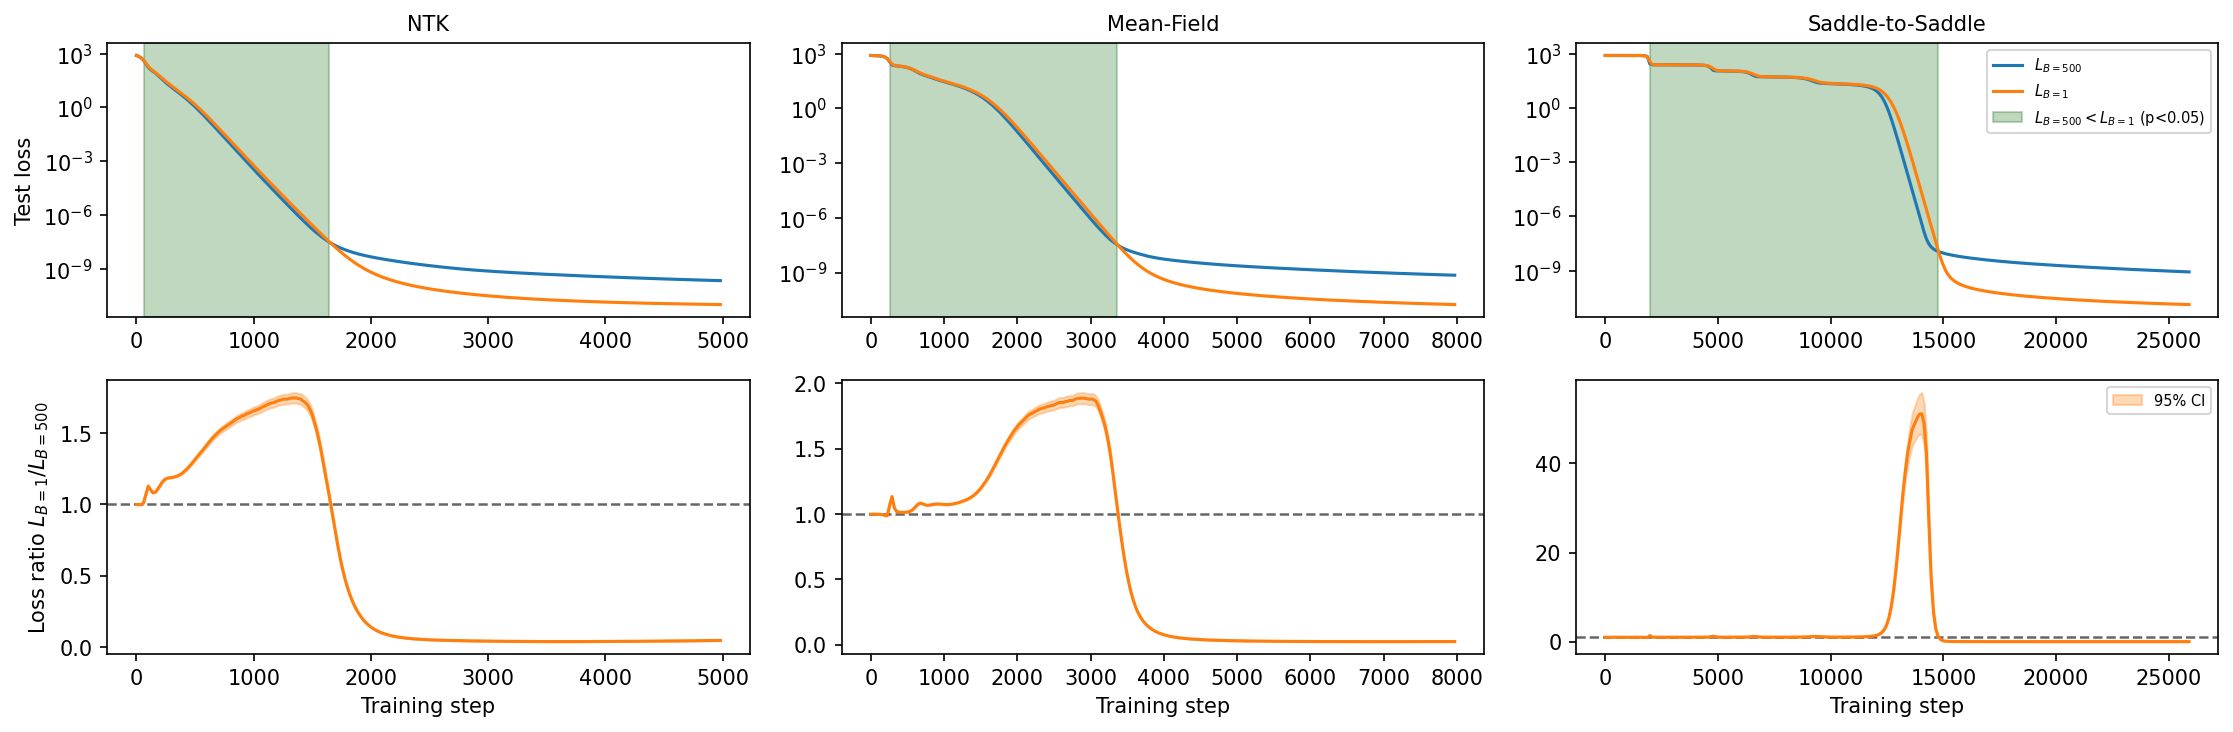
\includegraphics[width=\linewidth,height=0.56\textheight,keepaspectratio]{figures/DLN_losses_regimes.png}
    \end{figure}
\end{frame}

\begin{frame}{Singular values of student matrix}
    \begin{figure}
        \centering
        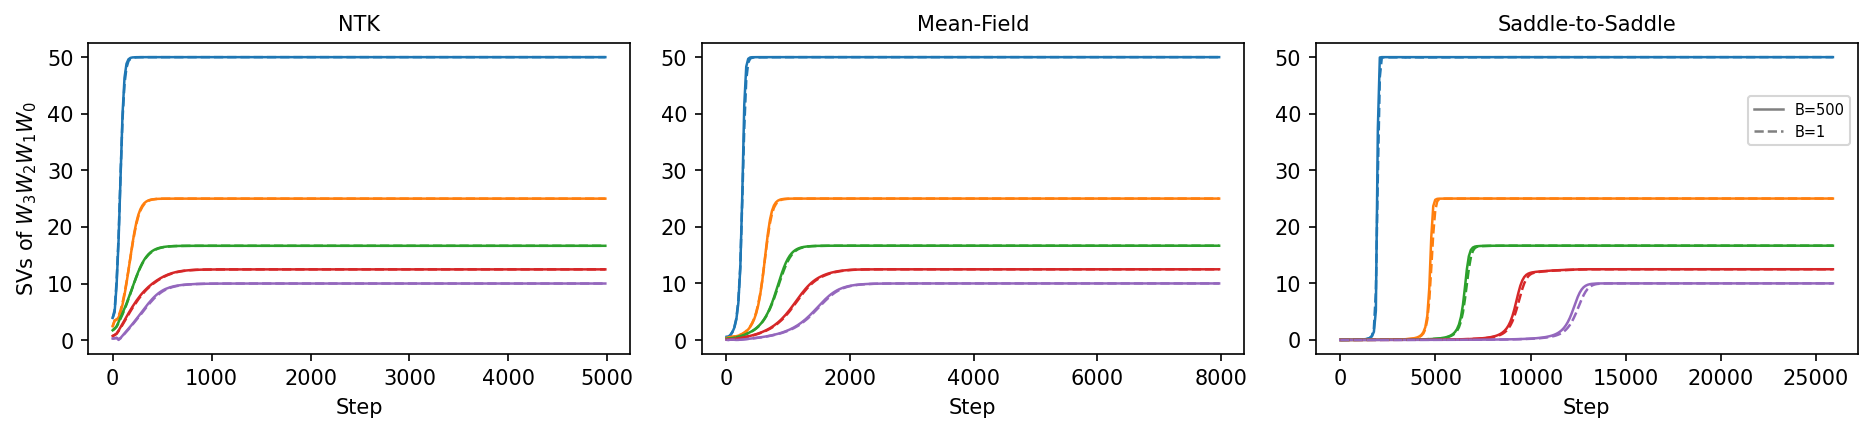
\includegraphics[width=\linewidth,height=0.75\textheight,keepaspectratio]{figures/DLN_sv_students.png}
    \end{figure}
\end{frame}

\begin{frame}{Singular values of individual weight matrices}
    \begin{figure}
        \centering
        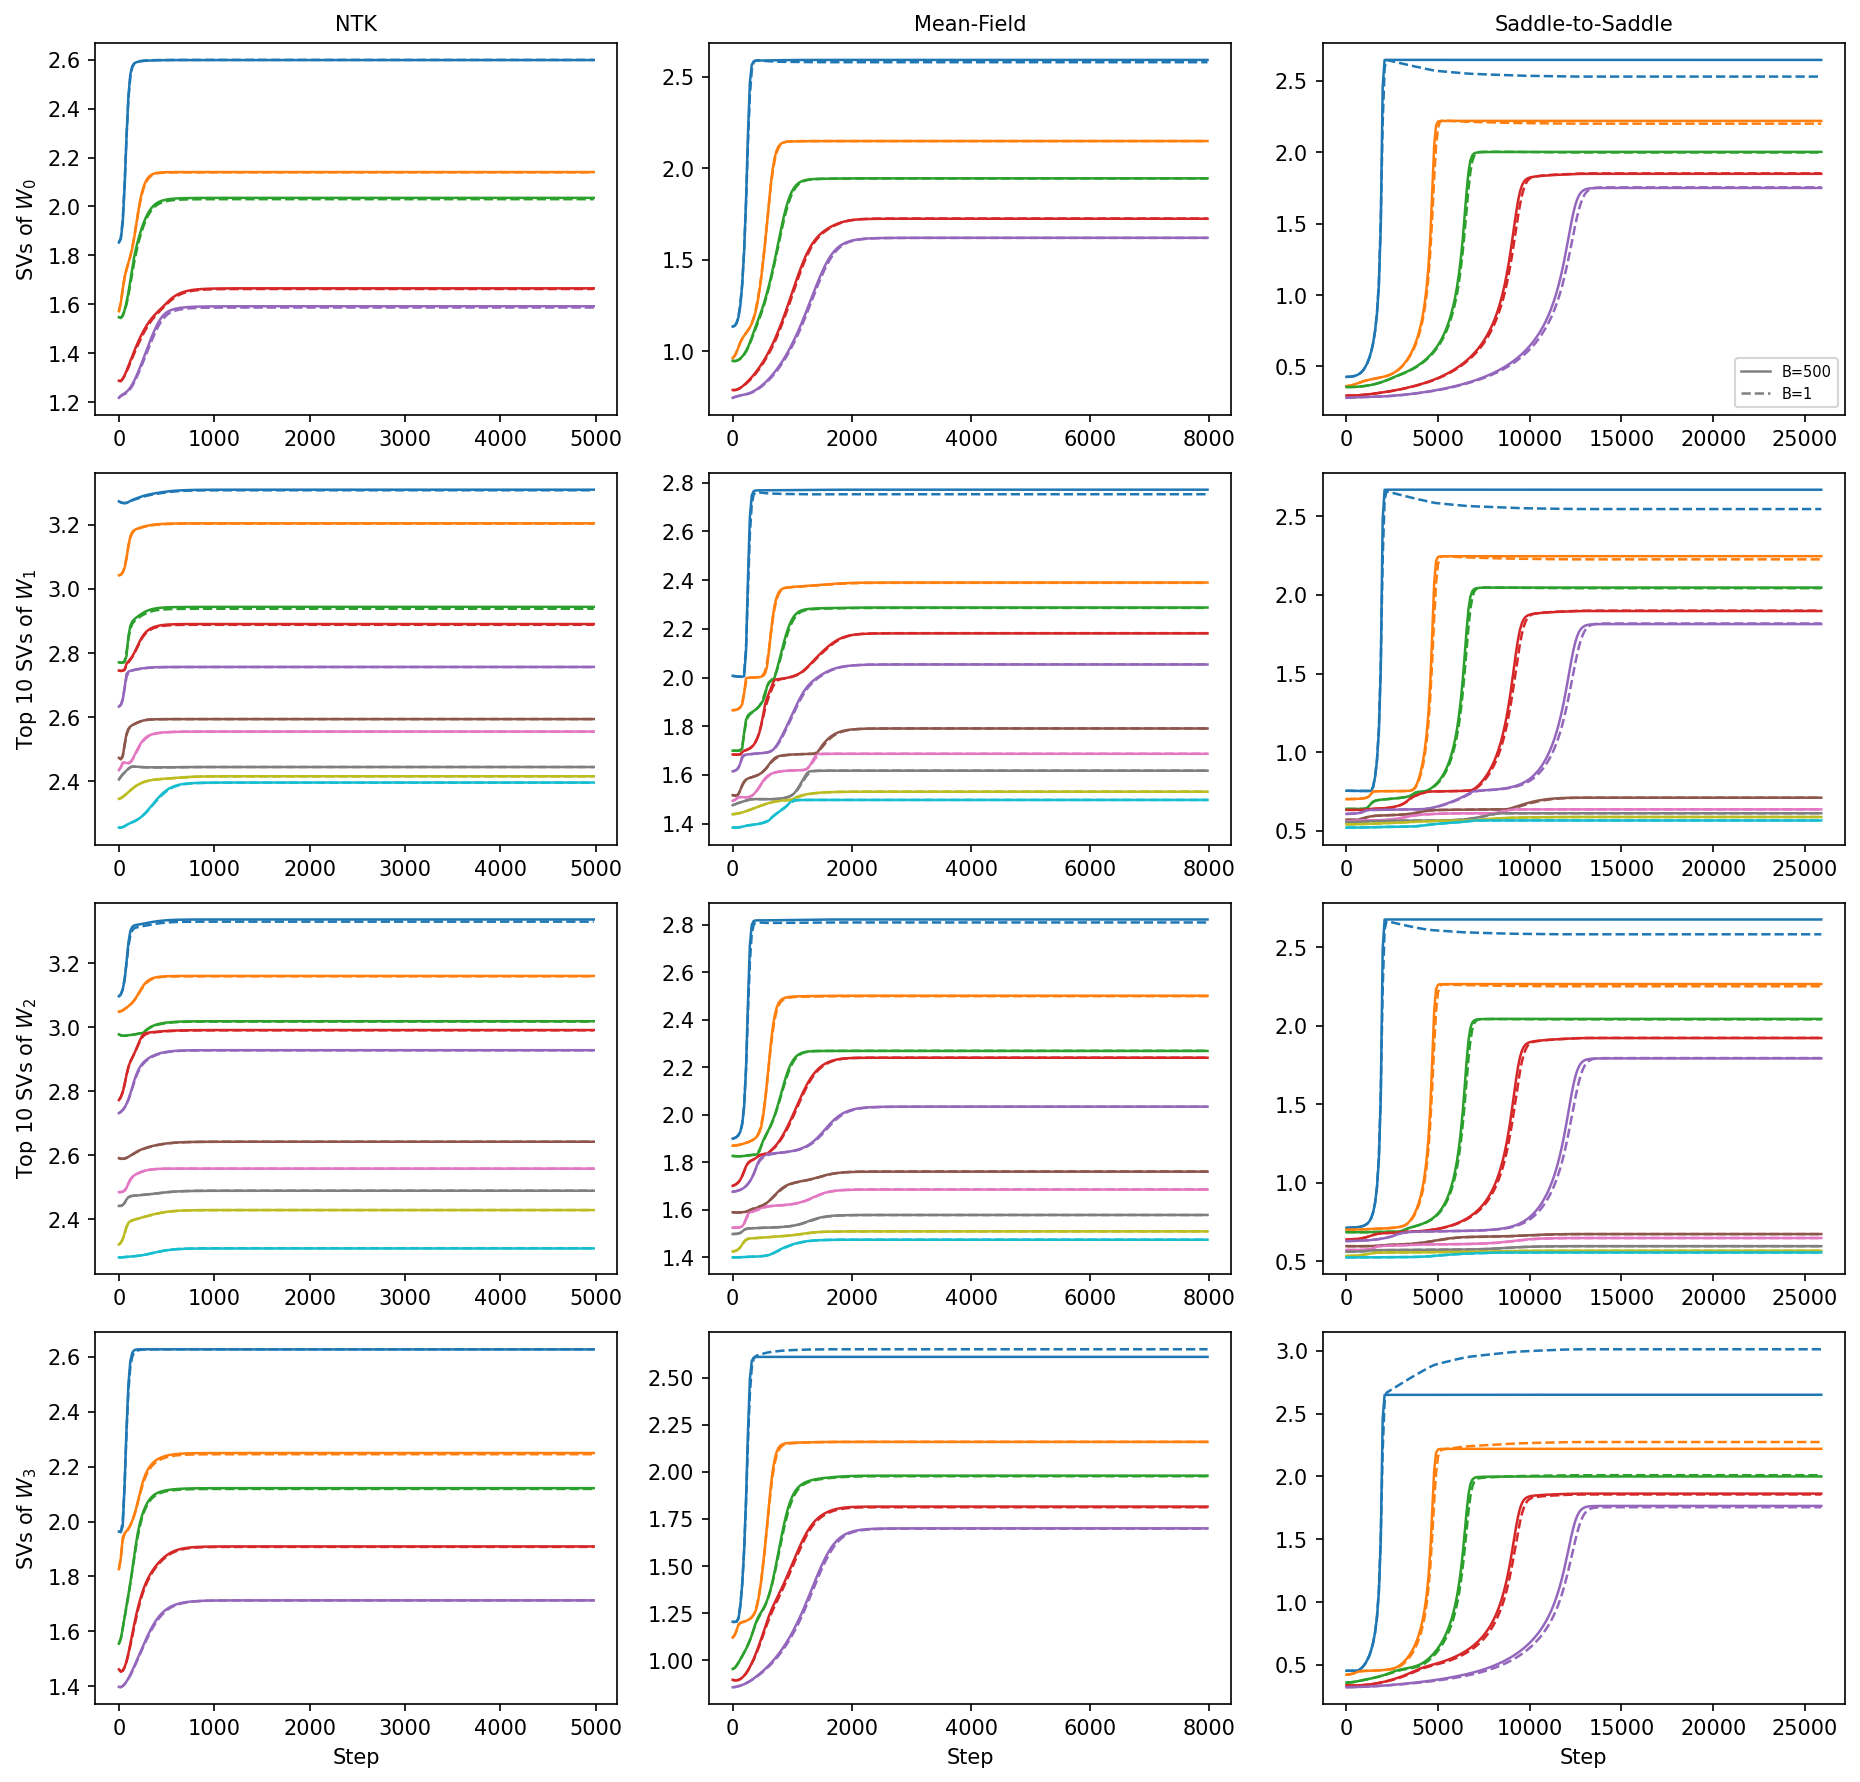
\includegraphics[width=\linewidth,height=0.75\textheight,keepaspectratio]{figures/DLN_individual_sv.png}
    \end{figure}
\end{frame}
\begin{frame}{Lazy Regime (NTK or Linear regime)}
  \small
  For a DLN of depth $L$ with initialization $\theta(0)\sim N(0,\sigma)$ and $\sigma^2 = d_L^{-\gamma}, \ \gamma < 1$:
  \[
    \dot{W} \approx K_0[M - W]
  \]

  Leading to the following solution:
  \[
    W(t) = M - \exp(-K_0 t)[M - W(0)]
  \]

  The time scale of learning is fixed by the NTK at initialization:
  \[
    t \approx -k_0^{-1}\log\left(\frac{s - w_f}{s - w_0}\right)
  \]

  Behaves like a shallow linear network
\end{frame}
\begin{frame}{Rich regime}
  \small
  For balanced and aligned weights (or $\gamma >1$), singular values of student satisfy:
  \[
    \dot{w}_{\alpha} = 2\left(s_{\alpha} - w_{\alpha}\right)w_{\alpha}.
  \]

  Solving this ODE for $w(t):=w_{\alpha}$ gives:
  \[
    w(t)=\frac{s}{1+\left(\frac{s}{w_0}-1\right)e^{-2s t}}.
  \]

  Timescale of learning
  \[
    t=\frac{1}{2s}\,\ln\!\left(\frac{w_f\,(s-w_0)}{w_0\,(s-w_f)}\right), \qquad s\neq 0.
  \]
\end{frame}
\begin{frame}{Takeaways}
  \begin{block}{Key points}
    \begin{itemize}
      \item Depth and specific initialization induce a sadde-to-saddle dynamics
      \item Gradient flow has a simplicity bias: low rank approximation
      \item Large initialization and width is NTK regime: no feature learning, NTK is frozen
      \item In saddle to saddle regime, time scale of learning set by the size of singular value of target function
    \end{itemize}
  \end{block}
\end{frame}
\begin{frame}{References}
    \begin{itemize}
        \item Saxe, Andrew M., James L. McClelland, and Surya Ganguli. A mathematical theory of semantic development in deep neural networks. \textit{Proceedings of the National Academy of Sciences} 116.23 (2019): 11537-11546.
        \item Jacot, Arthur, et al. Saddle-to-saddle dynamics in deep linear networks: Small initialization training, symmetry, and sparsity. \textit{arXiv preprint} arXiv:2106.15933 (2021).
        \item Dominé, Clémentine CJ, et al. From lazy to rich: Exact learning dynamics in deep linear networks. \textit{arXiv preprint} arXiv:2409.14623 (2024)
        \item Zhang, Yedi, Andrew Saxe, and Peter E. Latham. Saddle-to-Saddle Dynamics Explains A Simplicity Bias Across Neural Network Architectures. \textit{arXiv preprint} arXiv:2512.20607 (2025).
        \item Zhenfeng Tu, Santiago Tomas Aranguri Diaz, and Arthur Jacot. Mixed dynamics
in linear networks: Unifying the lazy and active regimes. \textit{Advances in Neural
Information Processing Systems}, 37:106059–106104, 2024.
    \end{itemize}
\end{frame}
\sectionframe{Stochasticity}

\begin{frame}{Langevin dynamics}
  \begin{itemize}
    \item SGD: Sample a batch from a dataset and compute the batch gradient
    \item Continuous model with $B_t$ Brownian
  \end{itemize}

  \[
    d\theta_t=-\nabla L(\theta_t)\,dt+\sqrt{\eta\,\Sigma(\theta_t)}\,dB_t,
  \]

  \begin{itemize}
    \item Gradient noise covariance $\Sigma(\theta_t)$ depends on geometry: it is anisotropic and state-dependent
  \end{itemize}
\end{frame}

\begin{frame}{Fokker-Planck: Boltzmann equilibria}
  \small
  The Fokker-Planck equation (for density $p(\theta,t)$) is a local conservation law:
  \[
    \begin{aligned}
      \partial_t p & := - \nabla\cdot j \\
      j &:=- \nabla L(\theta)p(\theta) - \frac{\eta}{2}\nabla^\top\left(\Sigma(\theta)p(\theta)\right)
    \end{aligned}
  \]

  Important special case:
  \begin{itemize}
    \item Stationary distribution: $\partial_tp^{\ast}(x,t) = 0$
    \item Thermal equilibrium: $j=0$
    \item White noise: $\Sigma=\sigma^2 I$
  \end{itemize}

  \[
    p^{\ast}(\theta) \propto \exp\left(-\frac{2}{\eta\sigma^2}L_N(\theta)\right) \ \text{Boltzmann}
  \]
\end{frame}

\begin{frame}{Noise anisotropy}
  \small
  \begin{itemize}
    \item In general, noise is anisotropic: it introduces a different implicit bias
    \item In function space, Langevin introduces a drift
  \end{itemize}

  \[
    \frac{\eta}{2}\operatorname{Tr}(\Sigma(\theta)H(\theta))
  \]

  \begin{itemize}
    \item Heuristic: bias toward flatter minima
    \item More:
      \begin{itemize}
        \item see Govind Menon \href{https://arxiv.org/abs/2602.12257}{On the implicit regularization of Langevin dynamics with projected noise}
        \item My \href{https://arxiv.org/html/2604.06366v1}{paper} with collaborators deriving Langevin on DLNs during the saddle-to-saddle regime
      \end{itemize}
  \end{itemize}
\end{frame}

\begin{frame}{Golden Path hypothesis}
  \small
  \begin{itemize}
    \item Lots of debate about the implicit bias of SGD noise
    \item Transient (drift dominated) vs low-loss regime (diffusion dominated):
  \end{itemize}

  \centering
  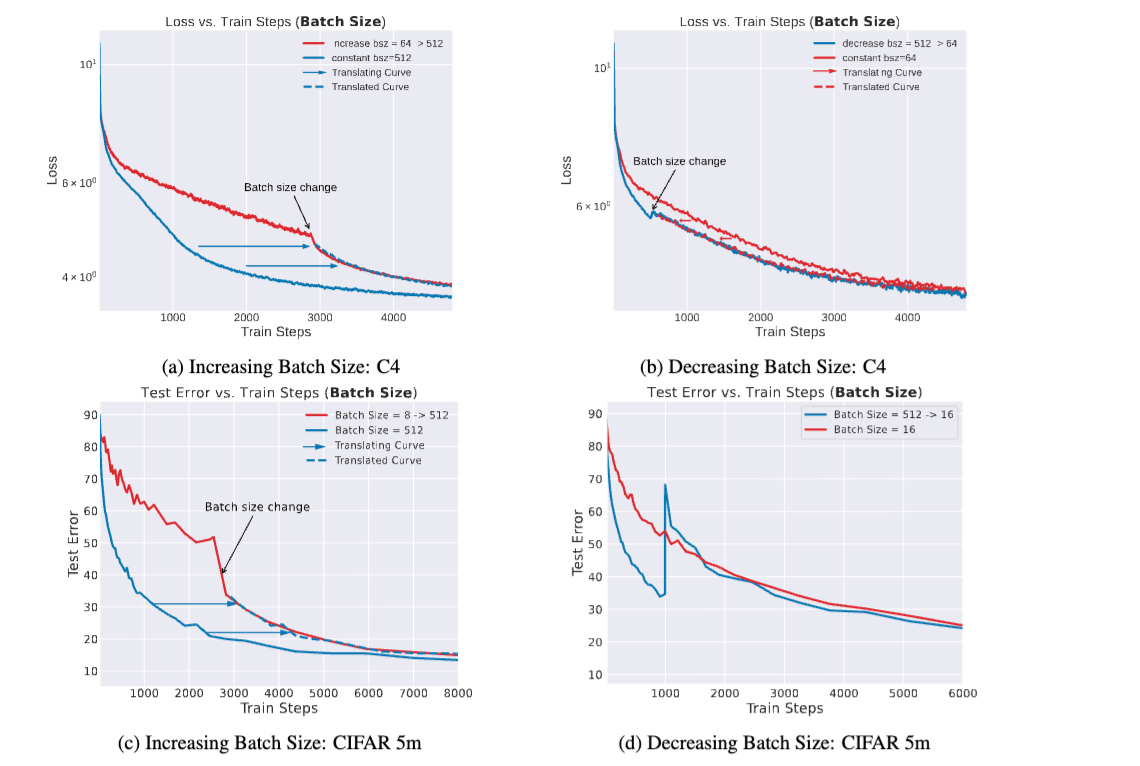
\includegraphics[height=0.6\textheight]{golden_path.png}

  \vspace{0.15cm}
  \footnotesize
  \emph{Beyond Implicit Bias: The Insignificance of SGD Noise in Online Learning}
\end{frame}
\sectionframe{Towards non linearity}

\begin{frame}{Neural race reduction}
  \centering
  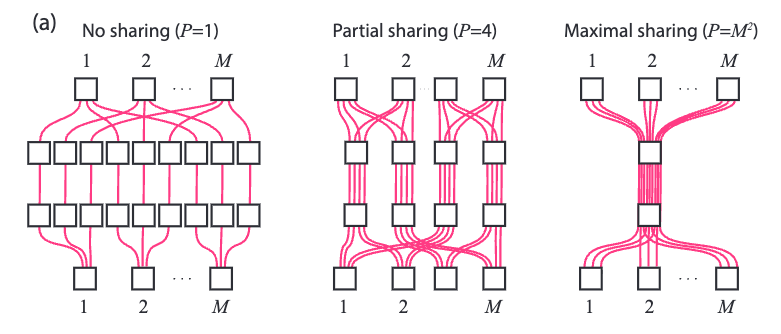
\includegraphics[height=0.68\textheight]{neural_race.png}

  \vspace{0.2cm}
  \footnotesize
  \emph{The Neural Race Reduction: Dynamics of Abstraction in Gated Networks, Andrew M. Saxe et al.}
\end{frame}

\begin{frame}{MLP and linear transformers}
  \small
  \emph{Saddle-to-Saddle Dynamics Explains A Simplicity Bias Across Neural Network Architectures, Saxe et al.}

  \vspace{0.2cm}
  \centering
  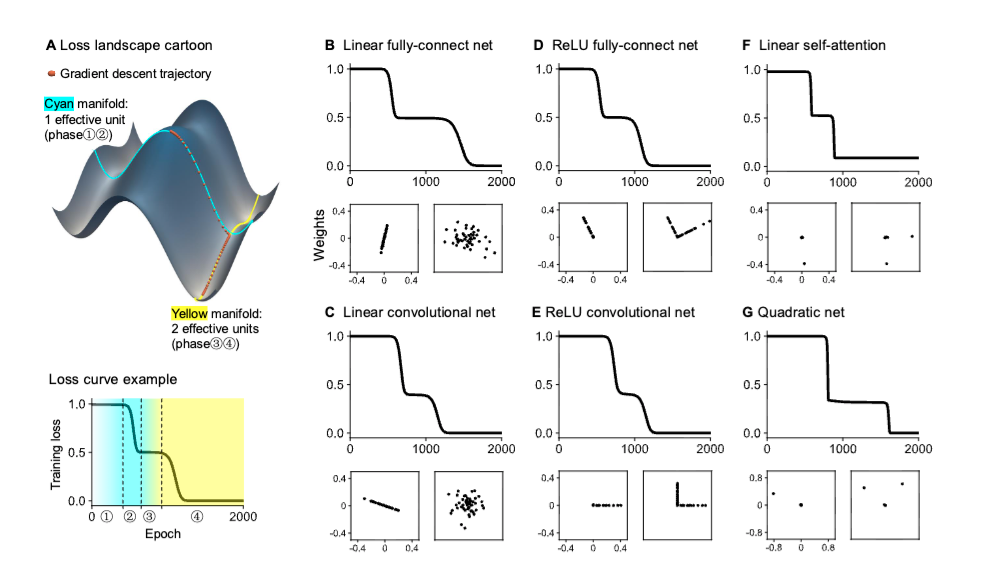
\includegraphics[height=0.58\textheight]{simplicity_bias_transformers_mlp.png}
\end{frame}
\begin{frame}{Takeaways}
  \begin{block}{Key points}
    \begin{itemize}
      \item SGD can be modelled via some SDE (with state dependent noise)
      \item If noise is white at thermal equilibrium the stationary distribution of the SDE is Boltzmann
      \item Implicit bias of Stochasticity not fully understood (flatness?) but more a 2nd order effect
      \item Non linearity can be modelled with gated DLN: neural race reduction
      \item MLP and linear transformers also have saddle to saddle dynamics
    \end{itemize}
  \end{block}
\end{frame}
\begin{frame}{Promising directions:}
\begin{itemize}
    \item Polynomial neural networks (quadratic activations)
    \item Related: Tensor and tree tensor networks
\end{itemize}
\begin{block}{Big questions}
\begin{itemize}
  \item Toy models of deep non linear learning
  \item Theory that capture natural data
  \item Making explicit the implicit biases of realistic Architectures
  \item Interplay between geometry and learning
  \item A statistical field theory of deep neural networks
  \item A more realistic theory of feature and hierarchical learning
\end{itemize}
\end{block}
Reference: \href{https://arxiv.org/abs/2604.21691}{\textit{There Will Be a Scientific Theory of Deep Learning, Jamie Simon et al.} }
\end{frame}
\end{document}
